% =====================================================================
% cap-02-arquitetura.tex — Capítulo 3: Arquitetura de Software
% =====================================================================

\chapter{Arquitetura de Software}
\label{cap:arquitetura}

Este capítulo descreve a arquitetura do sistema, organizada em cinco
seções: a justificativa do estilo arquitetural adotado
(Seção~\ref{sec:estilo}), a estrutura de módulos
(Seção~\ref{sec:modulos}), a máquina de estados que orquestra a execução
(Seção~\ref{sec:fsm}), as saídas visuais apresentadas ao operador
(Seção~\ref{sec:saidas}) e os padrões de projeto aplicados
(Seção~\ref{sec:patterns}).

\section{Estilo Arquitetural: Monolítico Modularizado}
\label{sec:estilo}

A arquitetura adotada é monolítica modularizada: todos os
módulos executam dentro de um único processo Python, comunicando-se por
chamada direta de função. A escolha foi norteada por três requisitos do
domínio:

\begin{description}
    \item[Latência mínima.] O \textit{loop} de Realidade Aumentada
          opera em mais de 30 quadros por segundo, e qualquer
          serialização ou marshalling intermediário (como em uma
          arquitetura de microsserviços) introduziria atraso intolerável
          entre a captura e a projeção.
    \item[Simplicidade de \textit{deploy}.] Um único ponto de entrada
          (\texttt{main.py}) e um conjunto fixo de dependências
          permitem operação \textit{plug and play} em qualquer máquina
          Windows ou Linux com Python e OpenCV instalados — condição
          explorada ao máximo pelo instalador offline descrito na
          Seção~\ref{subsec:instalador}.
    \item[Testabilidade.] Cada módulo encapsula uma responsabilidade
          bem definida, permitindo testes unitários isolados sem
          necessidade de \emph{mock} de rede ou \emph{containers}.
\end{description}

\subsection{Instalador \textit{offline} para Windows}
\label{subsec:instalador}

A operação em unidades de instrução militar deve considerar a possibilidade
de que o sistema seja utilizado por pessoal sem formação específica em desenvolvimento
de \textit{software}, bem como em ambientes sem conectividade constante à internet.
Nesse contexto, a configuração manual do ambiente Python e a instalação de suas dependências
podem representar uma barreira à utilização do sistema, uma vez que o comando \texttt{pip install},
utilizado para obter e instalar pacotes de software a partir de um repositório, normalmente
requer acesso à internet. Para eliminar essa barreira e simplificar a implantação, o projeto inclui,
na pasta \texttt{installer/} do repositório (Anexo~A), um instalador único e totalmente offline para
o sistema operacional Windows 10/11 de 64~\textit{bits}, gerado com o Inno~Setup a partir do script
\texttt{ARSandbox.iss}. Em um computador que possua apenas o sistema operacional Windows, sem os demais
pré-requisitos necessários à execução do sistema, o instalador realiza automaticamente, em sequência:


\begin{enumerate}
    \item Copia o código-fonte, o mapa GeoTIFF de exemplo e a
          documentação para \texttt{C:\textbackslash ARSandbox};
    \item Instala o Python~3.12 (reaproveitando uma instalação
          existente, se houver) e cria um ambiente virtual dedicado;
    \item Instala todas as dependências (NumPy, OpenCV, \texttt{rasterio},
          SciPy, CustomTkinter, \texttt{comtypes}, \texttt{pykinect2})
          a partir de \emph{wheels} pré-baixadas, embutidas no próprio
          instalador — nenhum acesso à internet é necessário nesta
          etapa;
    \item Aplica automaticamente, via \texttt{patch\_pykinect2.py}, os
          cinco patches de compatibilidade que permitem ao
          \texttt{pykinect2} — escrito originalmente para Python~2/3.6
          — funcionar em Python~3.12 (entre eles, a correção de
          \texttt{sizeof(tagSTATSTG)} e a substituição de
          \texttt{numpy.distutils}, descontinuado nas versões recentes
          do NumPy);
    \item Instala o Kinect for Windows Runtime v2.0, necessário
          para o driver do sensor mesmo fora de um ambiente de
          desenvolvimento;
    \item Executa um teste de fumaça dos módulos importados, registrando
          o resultado em um arquivo de \emph{log}, e cria os atalhos
          ``AR Sandbox'' e ``AR Sandbox --- Diagnóstico do
          Kinect'' no Menu Iniciar.
\end{enumerate}

\noindent O resultado é que um instrutor da Seção de Simulação da AMAN,
sem qualquer conhecimento prévio de Python, consegue colocar o sistema
em operação executando um único instalador e clicando em ``Avançar'' —
o mesmo princípio de \textit{plug and play} que orienta a cadeia de
\textit{fallback} do sensor (Seção~\ref{subsec:fallback}) aplicado,
aqui, à própria instalação do \textit{software}.

\section{Módulos do Sistema}
\label{sec:modulos}

A árvore de arquivos do projeto é apresentada a seguir:

\begin{lstlisting}[language=, caption={Estrutura de módulos do projeto.}, label=lst:tree]
PFC-2026/
+-- main.py                  # Orquestrador (FSM + mouse callback)
+-- kinect_sensor.py         # Camada de Hardware (KinectSensor)
+-- motor_caixao_areia.py    # Motor matematico (algebra + grade)
+-- mde_cartografia.py       # Adaptador de MDE (GeoTIFF + fallback)
+-- test_motor_caixao.py     # 83 testes unitarios automatizados
+-- DOCUMENTACAO_OFICIAL.md  # Documentacao academica completa
+-- README.md                # Guia de uso pratico
+-- relatorio_tcc/           # Esta pasta (relatorio LaTeX do PFC)
\end{lstlisting}

A Tabela~\ref{tab:modulos} resume a responsabilidade de cada módulo.

\begin{table}[!ht]
\centering
\caption{Responsabilidades dos módulos.}
\label{tab:modulos}
\begin{tabular}{lll}
\toprule
\textbf{Camada} & \textbf{Módulo} & \textbf{Responsabilidade} \\
\midrule
Hardware     & \texttt{kinect\_sensor.py}    & Captura da nuvem 3D, fallback, simulação \\
Lógica       & \texttt{motor\_caixao\_areia.py} & Álgebra linear, discretização, projeção \\
Dados        & \texttt{mde\_cartografia.py}  & Leitura de GeoTIFF, fallback gaussiano \\
Orquestração & \texttt{main.py}              & FSM, janelas, callback de \emph{mouse} \\
\bottomrule
\end{tabular}
\end{table}

\section{Máquina de Estados Finita}
\label{sec:fsm}

A execução do sistema é controlada por uma máquina de estados finita
(\textit{Finite State Machine} — FSM) com quatro estados principais e
transições determinísticas controladas por teclado. A
Figura~\ref{fig:fsm} ilustra o diagrama de estados.

\begin{figure}[!ht]
\centering
\begin{lstlisting}[language=, basicstyle=\ttfamily\footnotesize, frame=single]
        +------+               +-----------+
        | INIT |--inicializa-->|   IDLE    |
        +------+   recursos    +-----+-----+
                                     | tecla [C]
                                     v
                               +------------+
              tecla [C]  <-----| CALIBRACAO |
              +-----+          | (SVD+G-S)  |
              |     |          +-----+------+
              |     |                | sucesso
              |     |                v
              |     |          +-----+--------+
              |     +----------| AR_LOOP      |---tecla [Q/ESC]--> ENCERRAR
              |                |  (real-time) |
              +----------------+--------------+
\end{lstlisting}
\caption{Máquina de estados do orquestrador.}
\label{fig:fsm}
\end{figure}

\begin{description}
    \item[INIT.] Inicializa o \texttt{KinectSensor} (com cadeia de
          \emph{fallback}), carrega o \texttt{AdaptadorMDE} (com
          \emph{fallback} gaussiano), cria as duas janelas OpenCV e
          registra o \emph{callback} de \emph{mouse}.
    \item[IDLE.] Exibe o mapa de profundidade colorido enquanto aguarda
          o comando de calibração (tecla \texttt{C}). Permite
          encerramento imediato.
    \item[CALIBRACAO.] Em modo real, captura uma nuvem de pontos,
          executa SVD + Gram-Schmidt + montagem de $T$ + composição com
          $T_{\text{shift}}$ (Seção~\ref{subsec:T-shift}). Em modo
          simulação, atribui $T = I_4$ e configura a projeção que mapeia
          $[0, L_x] \times [0, L_y]$ na janela do projetor.
    \item[AR\_LOOP.] Executa, a cada \emph{frame}, o \textit{pipeline}
          completo: captura $\to$ transformação $\to$ discretização
          $\to$ comparação MDE $\to$ projeção Tsai $\to$ rasterização.
          Eventos de \emph{mouse} entre quadros modificam a grade de
          areia virtual (modo simulação).
\end{description}

\section{Saídas Visuais}
\label{sec:saidas}

O sistema apresenta ao operador duas janelas OpenCV
simultâneas, com propósitos distintos e complementares:

\begin{description}
    \item[\texttt{Projecao\_Areia}.] Destinada ao projetor
          físico suspenso sobre a mesa: exibe exclusivamente a malha
          contínua de quadrados coloridos (vermelho/azul/verde) que
          constitui o \emph{feedback} operacional. Nenhum texto ou
          elemento de interface é desenhado sobre essa janela durante a
          operação normal, para não contaminar a projeção sobre a
          areia.
    \item[\texttt{Gabarito\_MDE}.] Janela de controle do
          operador, exibida no monitor do computador (não no
          projetor). Mostra o \emph{heatmap} do MDE de referência que
          está sendo replicado, sobreposto a um HUD (\emph{Heads-Up
          Display}) semitransparente com a legenda de cores, o estado
          corrente da máquina de estados, o indicador de calibração
          (pendente, em cache ou recém-calculada) e a taxa de quadros
          por segundo.
\end{description}

\begin{figure}[!ht]
\centering
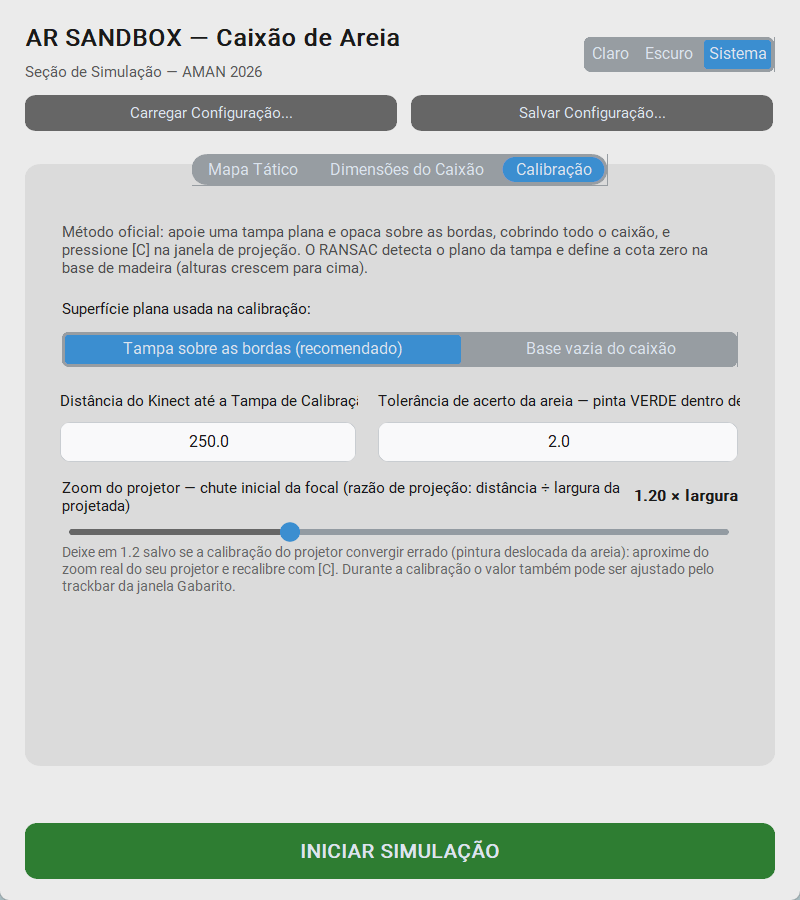
\includegraphics[width=0.75\textwidth]{img/gui_configuracao.png}
\caption{Interface gráfica de configuração inicial (CustomTkinter),
aba ``Calibração'': modo de calibração (tampa/base), distância do
Kinect à superfície de referência, tolerância de aceitação e o fator
inicial de zoom do projetor.}
\label{fig:gui-config}
\end{figure}

\subsection{Saída temporária de calibração: o tabuleiro quadriculado}
\label{subsec:saida-tabuleiro}

Durante a etapa opcional de calibração empírica do projetor
(via \texttt{calibrar\_projetor}, Seção~\ref{subsec:calib-empirica-projetor}), a janela
\texttt{Projecao\_Areia} deixa temporariamente de exibir a
malha de cores e passa a projetar um padrão de tabuleiro de
xadrez (\texttt{gerar\_imagem\_tabuleiro}) sobre a superfície de
referência. Essa saída é usada apenas enquanto dura a rotina de
calibração: uma câmera captura o tabuleiro projetado, a função
\texttt{encontrar\_cantos\_tabuleiro} detecta os cantos internos na
imagem capturada e \texttt{cv2.calibrateCamera} estima, por
otimização não linear, os parâmetros intrínsecos do projetor a partir
das correspondências entre cantos conhecidos e cantos detectados. Um
\textit{trackbar} de ajuste do fator de zoom/\textit{throw ratio}
(``\texttt{Zoom proj~x100}'') é exibido na janela \texttt{Gabarito\_MDE}
durante essa etapa, permitindo ao operador corrigir o chute inicial da
distância focal caso a otimização convirja para um mínimo local
incorreto. Encerrada a calibração — com sucesso ou por cancelamento —,
a janela \texttt{Projecao\_Areia} volta a exibir exclusivamente a
malha de cores. Este é, portanto, um mecanismo de depuração e
calibração assistida, e não uma saída destinada ao uso operacional
corrente do sistema; na configuração padrão, o sistema opera com os
parâmetros de projeção obtidos analiticamente
(Seção~\ref{sec:passo4}), e a rotina de tabuleiro permanece disponível
como caminho alternativo, já coberto pela suíte de testes
(Capítulo~\ref{cap:resultados}).

\section{Padrões de Projeto Aplicados}
\label{sec:patterns}

A Tabela~\ref{tab:patterns} elenca os padrões de projeto de
Gamma et al.~\citeonline{gamma1995design} identificados na implementação, e o
restante desta seção explica o propósito de cada um.

\begin{table}[!ht]
\centering
\caption{Padrões de projeto aplicados.}
\label{tab:patterns}
\begin{tabular}{lll}
\toprule
\textbf{Padrão} & \textbf{Onde} & \textbf{Propósito} \\
\midrule
Strategy + Fallback & \texttt{KinectSensor} & Seleção transparente de \textit{driver} \\
Adapter             & \texttt{AdaptadorMDE} & Isolar formato GeoTIFF da interface \\
State Machine       & \texttt{main.py}      & Controle determinístico do fluxo \\
Observer (Callback) & \texttt{main.py}      & Eventos de \emph{mouse} desacoplados \\
\bottomrule
\end{tabular}
\end{table}

\begin{description}
    \item[Strategy + \textit{Fallback} (\texttt{KinectSensor}).] Cada
          backend de captura (PyKinect2, Open3D, \texttt{freenect},
          simulação) implementa a mesma interface de
          \texttt{capturar\_nuvem()}, encapsulando um algoritmo de
          aquisição intercambiável — a essência do padrão
          \textit{Strategy}. A particularidade deste projeto é compor
          o \textit{Strategy} com uma cadeia de fallback
          (Seção~\ref{subsec:fallback}): em vez de o cliente escolher
          explicitamente a estratégia, o próprio construtor de
          \texttt{KinectSensor} tenta cada uma em ordem de preferência
          até que uma tenha sucesso, tornando a seleção do
          \textit{driver} transparente ao restante do sistema —
          \texttt{main.py} chama sempre o mesmo método, qualquer que
          seja o backend efetivamente ativo.
    \item[Adapter (\texttt{AdaptadorMDE}).] O formato de arquivo
          GeoTIFF, a biblioteca \texttt{rasterio} e a convenção de
          eixos cartográficos são detalhes de implementação que o
          restante do sistema não deveria conhecer. A classe
          \texttt{AdaptadorMDE} adapta essa interface heterogênea a um
          único método uniforme, \texttt{obter\_z\_alvo(x, y)}, que
          devolve a altura de referência em coordenadas físicas da
          mesa — seja a origem um GeoTIFF real, seja um mapa sintético
          de \textit{fallback} (Cubo Central ou Morro Gaussiano).
    \item[\textit{State Machine} (\texttt{main.py}).] A execução é
          modelada como uma enumeração explícita de estados
          (Seção~\ref{sec:fsm}) com transições determinísticas
          disparadas por eventos de teclado. Esse padrão evita a
          alternativa comum de controlar o fluxo por variáveis
          booleanas soltas (\emph{flags}), que tendem a
          produzir estados inválidos ou inconsistentes à medida que o
          programa cresce; aqui, o estado corrente é sempre um único
          valor da enumeração \texttt{Estado}, tornando impossível,
          por construção, que o sistema esteja simultaneamente
          calibrando e em \textit{loop} de Realidade Aumentada.
    \item[\textit{Observer} via \textit{callback} (\texttt{main.py}).]
          Os eventos de \emph{mouse} (pressionar, arrastar, soltar os
          botões) são registrados por \texttt{cv2.setMouseCallback} e
          notificados de forma assíncrona à função de tratamento, que
          atualiza o estado persistente da areia virtual
          (Seção~\ref{sec:emulador}) sem que o \textit{loop} principal
          precise consultar ativamente (\emph{polling}) a posição do
          cursor a cada quadro — um desacoplamento típico do padrão
          \textit{Observer}, aqui implementado pelo mecanismo nativo
          de \textit{callbacks} do OpenCV em vez de uma hierarquia
          explícita de classes \textit{Subject}/\textit{Observer}.
\end{description}

\subsection{Cadeia de \textit{fallback} do sensor}
\label{subsec:fallback}

O construtor do \texttt{KinectSensor} executa, em ordem, quatro
tentativas de inicialização. A primeira que tiver sucesso é mantida; em
caso contrário, prossegue-se ao próximo nível. A
Figura~\ref{fig:fallback} esquematiza a cadeia.

\begin{figure}[!ht]
\centering
\begin{lstlisting}[language=, basicstyle=\ttfamily\footnotesize, frame=single]
1. PyKinect2 (SDK Microsoft - Kinect v2)        ---falhou--> 2
2. Open3D    (Azure Kinect / RealSense)         ---falhou--> 3
3. freenect  (Kinect v1 / libfreenect)          ---falhou--> 4
4. SIMULACAO (grade persistente + pa virtual)   <-- sempre OK
\end{lstlisting}
\caption{Cadeia de \textit{fallback} do \texttt{KinectSensor}.}
\label{fig:fallback}
\end{figure}

A garantia operacional fundamental é que o sistema nunca falha
catastroficamente por ausência de hardware: o quarto nível
(Simulação) é puramente computacional e não depende de
quaisquer recursos externos. Garantia análoga aplica-se ao
\texttt{AdaptadorMDE}: na ausência ou falha de leitura do GeoTIFF, é
gerada uma superfície gaussiana sintética que assegura visualização
significativa para a audiência.
